\chapter{Theoretical Background}

In this chapter we will present a brief introduction to neural networks and then describe the underlying concepts of the Convolutional Neural Network (CNN).
We will focus on presenting the main concepts that will be used in the development of pose estimation algorithms.

\section{Neural network}

In the Neural Networks chapter, we will talk in the first part about a brief history, presenting the three periods through which artificial intelligence has passed.
Then we will address the biological part that is found in neural networks.
In the next section we will discuss what is a neural network , how many types of such networks are there? What is a neuron? But an activation function?
Finally, we will discuss learning such a neural network with its specific algorithms.

\subsection{History}
Artificial intelligence takes us to think of some SF films, 
but it still has a long way to go, for now these intelligent algorithms can
only get to the level of intelligence of an insect, 
they work better in certain exact tasks as imagine detectie  and not in general like a brain.

But let's not forget that this domain has been built around the dream to overcome human intelligence.
The essential question is whether such a system can be implemented on a computer?

The domain of psychology was the first to have had the artificial intelligence applicability, 
the most famous Turing test that appeared in 1950. 
It involves a conversation of a person with a computer and another person and he has to guess who is the person. \cite{historyofneuronalnetwork}

Three great periods are in the history of artificial intelligence. 
In the first period, only after the Second World War. The first programs that implement various smart algorithms to solve puzzles. \cite{historyofneuronalnetwork}

An important algorithm in this field is Samuels' game, it was quite simple to implement. They save certain winning positions throughout the game.\cite{historyofneuronalnetwork}
The first period kept until 1965, but no algorithm has led to major changes in people's lives. \cite{historyofneuronalnetwork}

In the second period, it focuses on the processing of natural language so many applications
 are launched that implement concepts from the processing of natural language.
 
One of the famous programs of those times was called ELIZA. This program learns to copy the conversations of a psychologist with his patients.
How did ELIZA work? 
ELIZA had a knowledge base in English and a field of psychology made up of a set of rules,  
so ELIZA worked on the "fit" principle.
For example, when it found the word "father," it said, "Tell me about your family" \cite{historyofneuronalnetwork}

 Also during this period, rule-based expert systems appeared. 
One such system was called MYCIN, which was designed to diagnose infectious diseases of the blood and recommend medical treatment. It is based on the rules made by specialists. \cite{historyofneuronalnetwork}

From 1975 to the present, there is the third period of artificial intelligence. 
This domain is becoming more stable and the industry adopting these intelligent systems.

Warren McCulloch and Walter Pitts have been the first research that has made the research. 
In 1940, they highlighted the first digital model of a neuron that discovers the computational capacity, 
also providing a mathematical abstraction of this concept.
Thus the synapses that a neuron makes through dendrites become inputs, 
the body of a neuron becomes an activation function, the axon has become the output and 
the BAIS notion has been introduced for mathematical restlessness features. \cite{historyofneuronalnetworkstanford}


In 1969, authors Marvin Minsky and Seymor Papert published the book "Perceptrons," which highlighted the limitations that exist for one-level neural networks.
After this publication many people who doing research was quit. \cite{historyofneuronalnetworkstanford}

Neural networks have become one of the most used in our days. 
Big Cloud companies offer an API through which any developer can get his own training in the easiest way.
 
\subsection{Biological}

The great mystery of this universe is the way people think, knowing for several 
thousand years that powerful head shots can generate loss of consciousness or even death.
But more than that, we know our brain is different from animals. 
In about 335 BC, Aristotle wrote, "Of all animals, man has the greatest brain." \cite{book.neuronal.network.1995}

The nervous system is made up of neurons. Each neuron can be represented as a unit.
Between neurons there are synapses that can be of two axo-somatic or axo-dendritic types. 
The body of the neuron has two types of extensions \cite{book.anatomie.1985}:
\begin{itemize}
\item Dentrites are relatively short, and branched near the cell
\item The axon is longer and thicker in the propagation of the electrical impulse.
\end{itemize}

\begin{figure}[htbp]
	\centerline{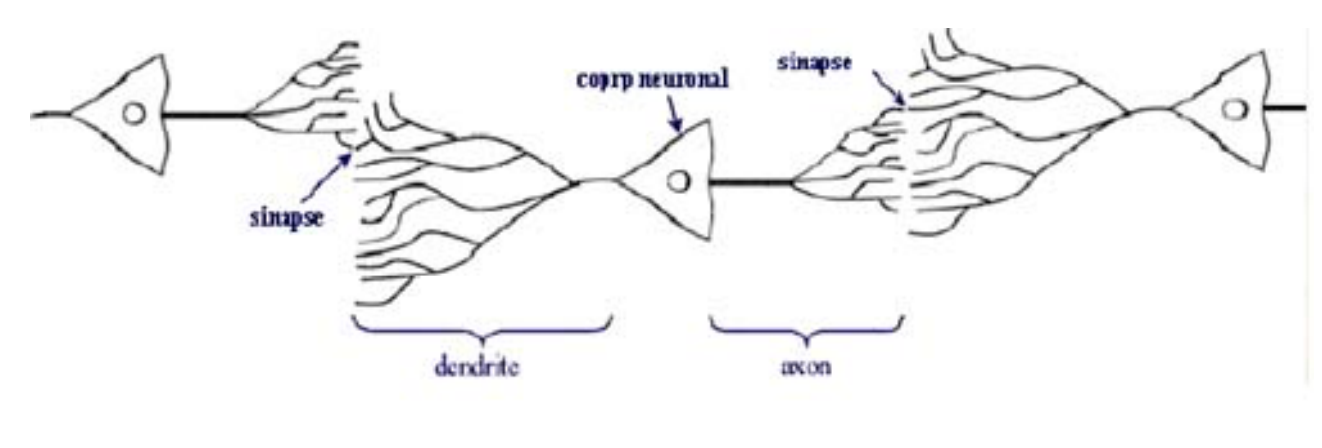
\includegraphics[scale=0.75]{fig/neuron.png}}  
	\caption{Network of biological neurons}
\end{figure}

While a reader uses a network of  $10^{11}$ biological neurons and $10^{4}$ connections between neurons, 
the processing time of $10^{-3}$ ms and $10^{-9}$ ms for electronic circuits, 
although biological neurons are more slower than electronic circuits, biological ones can process information much faster than any other circuit. \cite{book.anatomie.1985}
\subsection{Overview}

A neural network is a copy of the biological model, so it has nodes that are connected by links,
these links are actually real numbers that represent the memory of a network. 
Learning a neural network is accomplished by changing the weight between the nodes.

Any neural network is organized on layers, so there is an input layer and an output layer.
The input layer is the one that receives the data from the outside and 
the output layer provides us with the information we expect. \cite{book.neuronal.network.1995}

\begin{figure}[htbp]
	\centerline{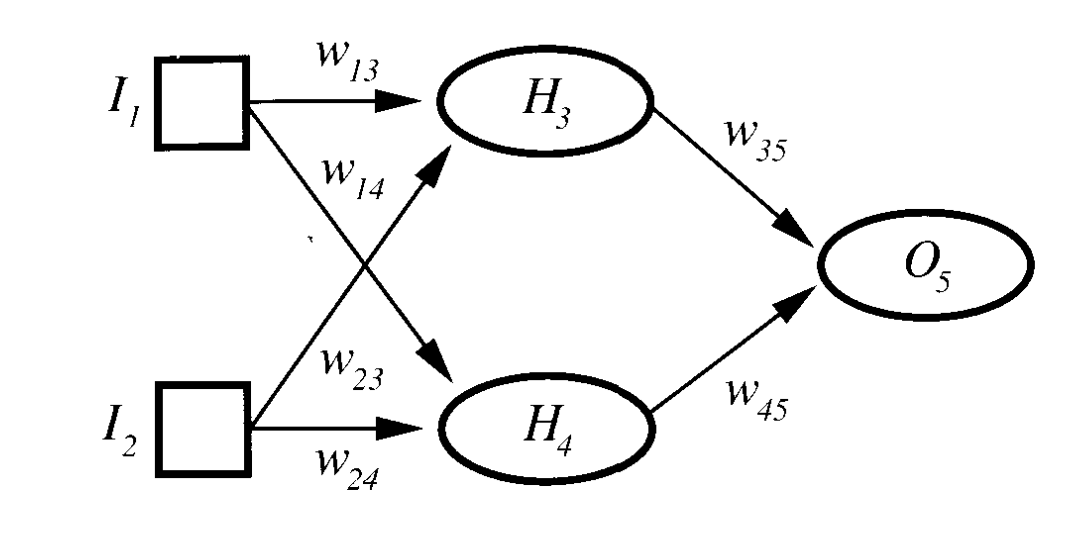
\includegraphics[scale=0.75]{fig/neuronal-network.png}}  
  \caption{Feedforward neural network  \cite{book.neuronal.network.1995}}
  \label{fig:feedforward}
\end{figure}

In Figure \ref{fig:feedforward} shows a neural network of the three-layer feed-forward type, which has links between the neurons in one direction,
because the cycles in such a network are missing, 
the calculation can continue evenly from the input nodes to the exit ones \cite{book.neuronal.network.1995}.

We can say that everything is summed up to the calculations of a value using input values, weights on each layer,
and activation function, most of the times it is difficult to choose the activation function or other parameters that make the performance of a network increase.

If we compare the human brain to such a network, we can see that some regions in the brain are feed-forware, but others do not, with quick back links. 
Then we can say that the human brain is closer to recurrent networks. \cite{book.neuronal.network.1995}.

\begin{figure}[htbp]
	\centerline{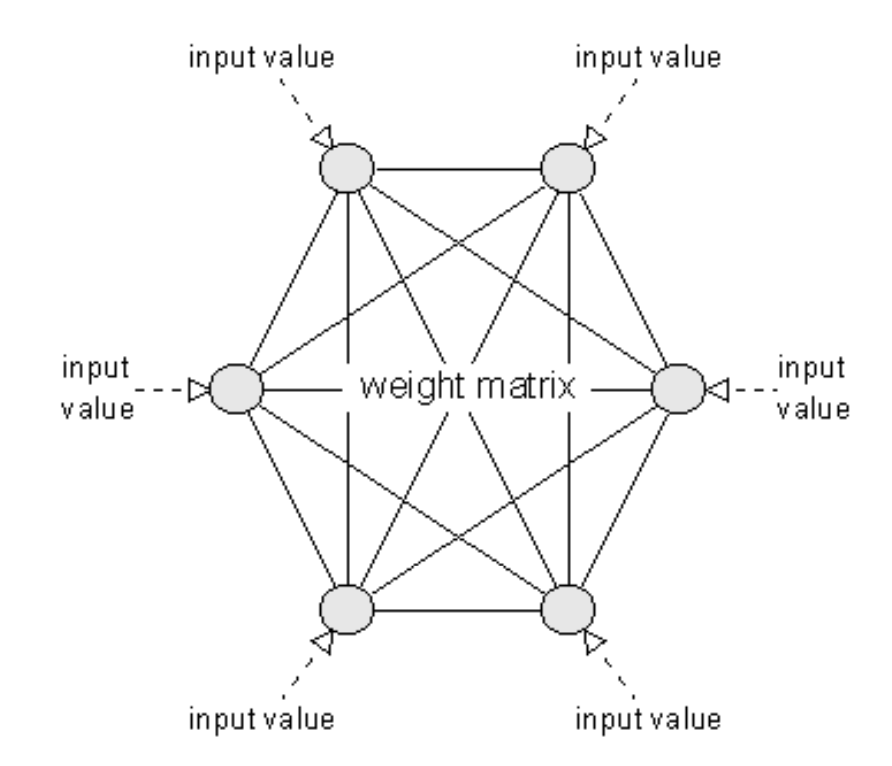
\includegraphics[scale=0.75]{fig/reatea-recurenta.png}}  
  \caption{Recurrent Networks - Hopfield  \cite{book.neuronal.network.1995}}
  \label{fig:hopfield}
  
\end{figure}

\par The best-understood neural networks of the recurrent type are thought to be Hopfield networks.
 Figure \ref{fig:hopfield} shows such a network. It can be observed that they use bidirectional connections between neurons, 
 the weights of the neurons being symmetrical. Besides, all layers in the network are both input and output, and the activation function is the sign function. 
Such a network functions as an associative memory.

Regarding the structure of the network, sometimes the performance of the network is very much dependent on this, 
because if we choose the wrong structure of a network then its performance will be poor. For example, if we choose a network too small, 
the mathematical model will not be representative of the training data,
 and if we choose too much a network, it will learn the training data well, memorizing them but will not be able to generalize the new entries. \cite{book.neuronal.network.1995}


 \begin{figure}[htbp]
	\centerline{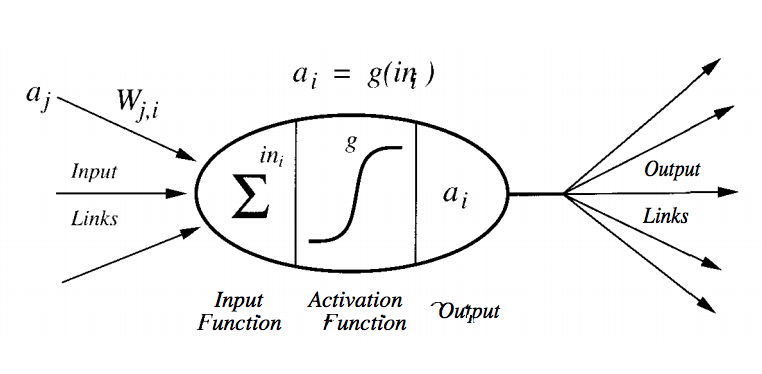
\includegraphics[scale=0.75]{fig/un-neuron.png}}  
  \caption{An artificial neuron  \cite{book.neuronal.network.1995}}
  \label{fig:anneuron}
  
\end{figure}

On top we will describe how a neuron works. Each neuron is connected to other neurons, 
some of them being input and others output, they make a relatively simple calculation, 
this computation being divided into two components, one linear and another non-linear. 
The first is a weighted sum of the input values in the neuron, this is the linear component and the 
second component is represented by the activation function, g, $a_i$
it converts the weighted sum to the final value, which then serves as an activation value units,
 most of the times the entire network uses the same activation function \cite{book.neuronal.network.1995}. 


 There are different models for the activation function, but only three of them are the most used, step function,
  sign and sigmoid, shown in Figure \ref{fig:activation-fun}. These activation functions allow the network to model nonlinear relationships between input parameters and output values. The step function returns the values according to a threshold t if the value is greater than the return threshold 1 and otherwise 0. There is also a biological motivation for this function, 1 represents the transmission of the nerve impulse and 0 the transmission failure.

  \begin{figure}[htbp]
    \centerline{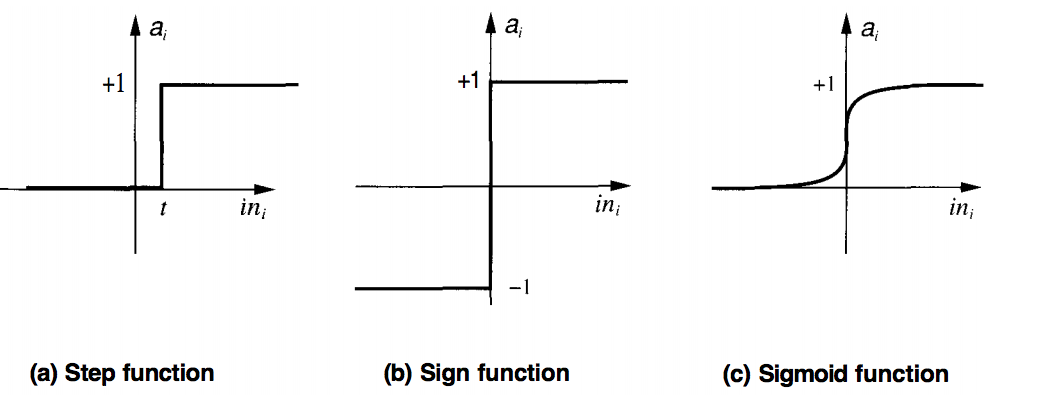
\includegraphics[scale=0.75]{fig/activation-fun.png}}  
    \caption{Activation functions \cite{book.neuronal.network.1995}}
    \label{fig:activation-fun}
    
  \end{figure}
  Another important issue is networking,
   their ability to learn by interacting with the environment is the main feature of the neural network. 
   One of the most popular algorithms is back-propagation. 
   We dedicated a special section below for the backpropagation algorithm. The idea behind learning algorithms is based on updating the weights, if there is an error between the output of the network and the value we expect, then weigh the weight so that it reduces the error, dividing it equally between the weights.

\subsection{Back propagation algorithm}

\section{Convolutional Neural Network}
\subsection{What is differente?}


% \section{The purpose of the application}